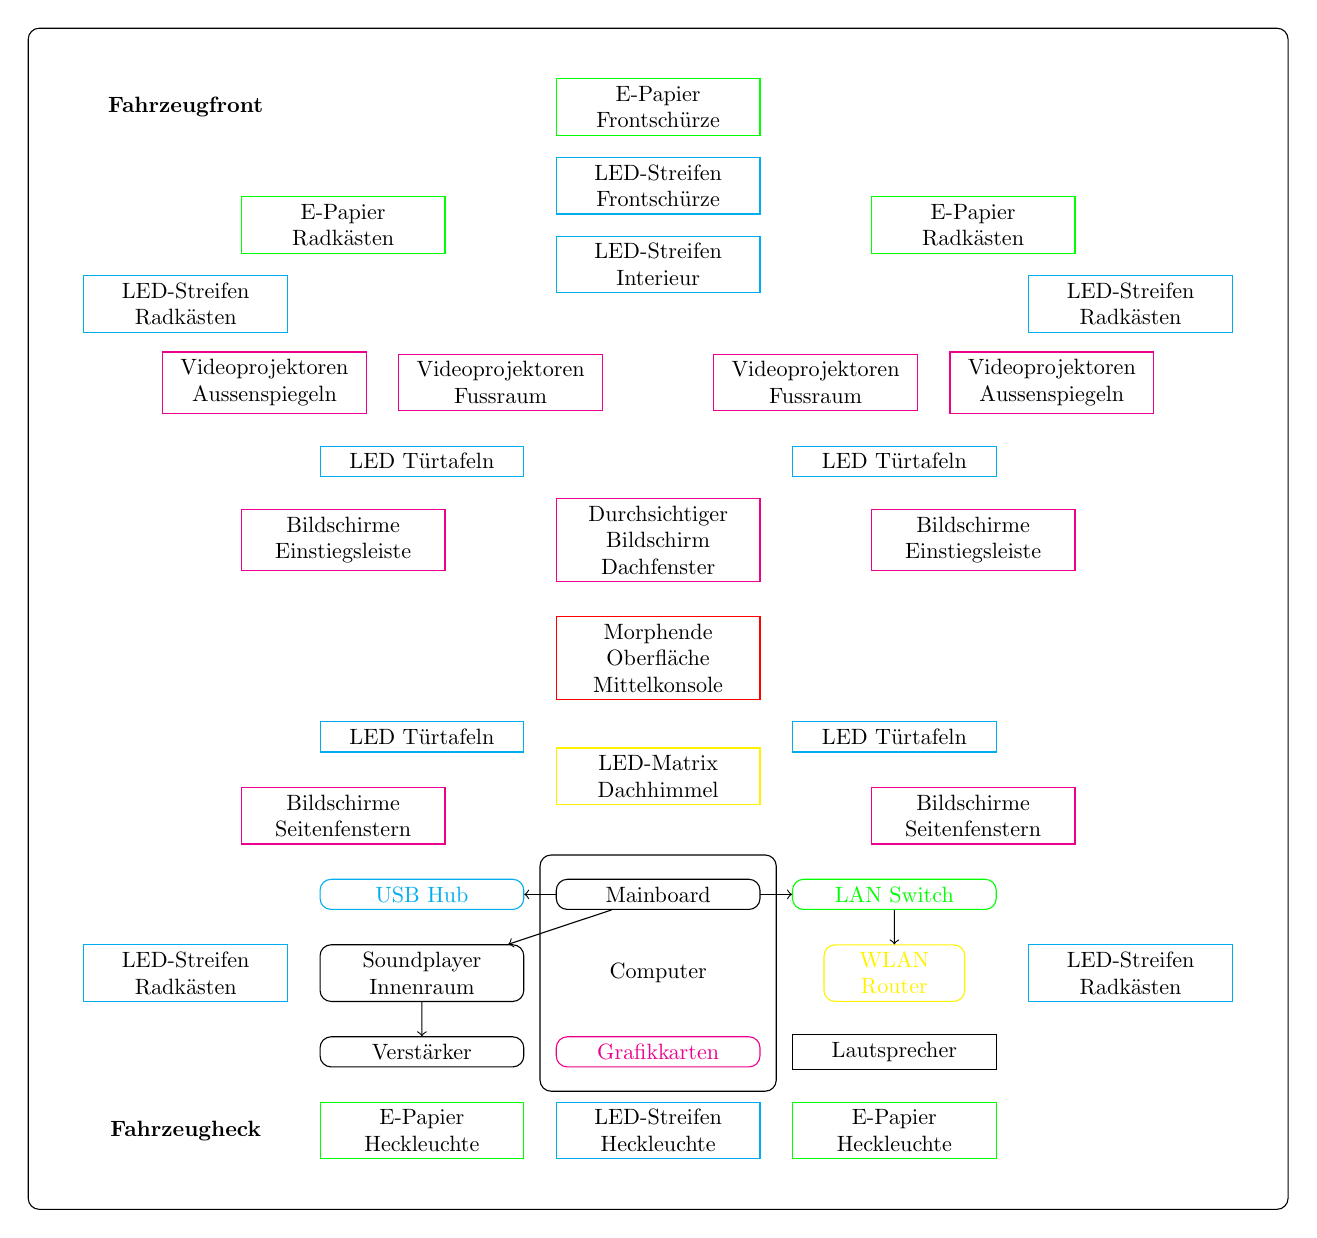
\begin{tikzpicture}[every node/.style={scale=0.8}]
	\node[text width=3.2cm, align=center] (Computer) at (0, -3) {Computer};
	\draw[draw=black, rounded corners] (-1.5,-4.5) rectangle ++(3,3);
	\node[draw, rectangle, text width=3cm, align=center, rounded corners] (Mainboard) at (0, -2) {Mainboard};
	\node[draw, rectangle, text width=3cm, align=center, rounded corners, magenta] (Grafikkarten) at (0, -4) {Grafikkarten};
	\node[draw, rectangle, text width=3cm, align=center, rounded corners, green] (LAN Switch) at (3, -2) {LAN Switch};
	\node[draw, rectangle, text width=2cm, align=center, rounded corners, yellow] (WLAN Router) at (3, -3) {WLAN Router};
	\node[draw, rectangle, text width=3cm, align=center, draw=green] (E-Papier Frontschrze) at (0, 8) {E-Papier Frontschürze};
	\node[draw, rectangle, text width=3cm, align=center, draw=cyan] (LED-Streifen Frontschrze) at (0, 7) {LED-Streifen Frontschürze};
	\node[draw, rectangle, text width=3cm, align=center, draw=green] (E-Papier Radksten) at (-4, 6.5) {E-Papier Radkästen};
	\node[draw, rectangle, text width=3cm, align=center, draw=green] (E-Papier Radksten2) at (4, 6.5) {E-Papier Radkästen};
	\node[draw, rectangle, text width=3cm, align=center, draw=cyan] (LED-Streifen Radksten) at (-6, 5.5) {LED-Streifen Radkästen};
	\node[draw, rectangle, text width=3cm, align=center, draw=cyan] (LED-Streifen Radksten) at (6, 5.5) {LED-Streifen Radkästen};
	\node[draw, rectangle, text width=3cm, align=center, draw=cyan] (LED-Streifen Radksten) at (-6, -3) {LED-Streifen Radkästen};
	\node[draw, rectangle, text width=3cm, align=center, draw=cyan] (LED-Streifen Radksten) at (6, -3) {LED-Streifen Radkästen};
	\node[draw, rectangle, text width=3cm, align=center, draw=magenta] (Videoprojektoren Aussenspiegeln) at (5, 4.5) {Videoprojektoren Aussenspiegeln};
	\node[draw, rectangle, text width=3cm, align=center, draw=magenta] (Videoprojektoren Aussenspiegeln) at (-5, 4.5) {Videoprojektoren Aussenspiegeln};
	\node[draw, rectangle, text width=3cm, align=center, draw=magenta] (Bildschirme Seitenfenstern) at (-4, -1) {Bildschirme Seitenfenstern};
	\node[draw, rectangle, text width=3cm, align=center, draw=magenta] (Bildschirme Seitenfenstern) at (4, -1) {Bildschirme Seitenfenstern};
	\node[draw, rectangle, text width=3cm, align=center, draw=cyan] (LED-Streifen Heckleuchte) at (0, -5) {LED-Streifen Heckleuchte};
	\node[draw, rectangle, text width=3cm, align=center, draw=green] (E-Papier Heckleuchte) at (-3, -5) {E-Papier Heckleuchte};
	\node[draw, rectangle, text width=3cm, align=center, draw=green] (E-Papier Heckleuchte) at (3, -5) {E-Papier Heckleuchte};
	\node[draw, rectangle, text width=3cm, align=center, draw=cyan] (LED-Streifen Interieur) at (0, 6) {LED-Streifen Interieur};
	\node[draw, rectangle, text width=3cm, align=center, draw=cyan] (LED Trtafeln) at (-3, 3.5) {LED Türtafeln};
	\node[draw, rectangle, text width=3cm, align=center, draw=cyan] (LED Trtafeln) at (3, 3.5) {LED Türtafeln};
	\node[draw, rectangle, text width=3cm, align=center, draw=cyan] (LED Trtafeln) at (-3, 0) {LED Türtafeln};
	\node[draw, rectangle, text width=3cm, align=center, draw=cyan] (LED Trtafeln) at (3, 0) {LED Türtafeln};
	\node[draw, rectangle, text width=3cm, align=center, draw=magenta] (Bildschirme Einstiegsleiste) at (-4, 2.5) {Bildschirme Einstiegsleiste};
	\node[draw, rectangle, text width=3cm, align=center, draw=magenta] (Bildschirme Einstiegsleiste) at (4, 2.5) {Bildschirme Einstiegsleiste};
	\node[draw, rectangle, text width=3cm, align=center, draw=magenta] (Videoprojektoren Fussraum) at (-2, 4.5) {Videoprojektoren Fussraum};
	\node[draw, rectangle, text width=3cm, align=center, draw=magenta] (Videoprojektoren Fussraum) at (2, 4.5) {Videoprojektoren Fussraum};
	\node[draw, rectangle, text width=3cm, align=center, draw=red] (Morphende Oberflche Mittelkonsole) at (0, 1) {Morphende Oberfläche Mittelkonsole};
	\node[draw, rectangle, text width=3cm, align=center, draw=magenta] (Durchsichtiger Bildschirm Dachfenster) at (0, 2.5) {Durchsichtiger Bildschirm Dachfenster};
	\node[draw, rectangle, text width=3cm, align=center, draw=yellow] (LED-Matrix Dachhimmel) at (0, -0.5) {LED-Matrix Dachhimmel};
	\node[draw, rectangle, text width=3cm, align=center, rounded corners] (Soundplayer Innenraum) at (-3, -3) {Soundplayer Innenraum};
	\node[draw, rectangle, text width=3cm, align=center, rounded corners, cyan] (USB Hub) at (-3, -2) {USB Hub};
	\node[draw, rectangle, text width=3cm, align=center, rounded corners] (Verstrker) at (-3, -4) {Verstärker};
	\node[draw, rectangle, text width=3cm, align=center] (Lautsprecher) at (3, -4) {Lautsprecher};
	\draw[->] (Mainboard) -> (LAN Switch);
	\draw[->] (LAN Switch) -> (WLAN Router);
	\draw[->] (Mainboard) -> (Soundplayer Innenraum);
	\draw[->] (Mainboard) -> (USB Hub);
	\draw[->] (Soundplayer Innenraum) -> (Verstrker);
	\draw[rounded corners] (0, 9) -- (8,9) -- (8,-6) -- (-8,-6) -- (-8,9) -- (0,9);
	\node at (-6,8) {\textbf{Fahrzeugfront}};
	\node at (-6,-5) {\textbf{Fahrzeugheck}};
\end{tikzpicture}